\section{Recurrent Neural Networks}
\label{back:rnn}

Alongside \acrshort{cnn}s which have become immensely popular due to their applications especially within computer vision \cite{oshea2015introduction}, \acrfull{rnn} is a type of \acrfull{ann} more suited for time series data, speech recognition and various other tasks. Where as \acrfull{cnn} networks performs convolutions on the data, not taking into account values at previous timesteps, \acrshort{rnn} cells work on one datapoint at a time, being influenced by previous values.
 They have regained more popularity due to its successful applications with sequential data \cite{karpathy2015visualizing}, yet have been studied for about 80 years. In late

The main advantage of \acrshort{rnn} comes from their ability to remember previous values, and perform calculations where these are favored

The building blocks of an \acrshort{rnn} is the recurrant neuron. They take an input $x_t$ at time $t$, with the state at previous time step $h_{t-1}$ and produces the next time step. 


\begin{equation}
    h_t = f(W_hh_{t-1}+W_xx_t)
\end{equation}

\begin{figure}[h]
    \centering
    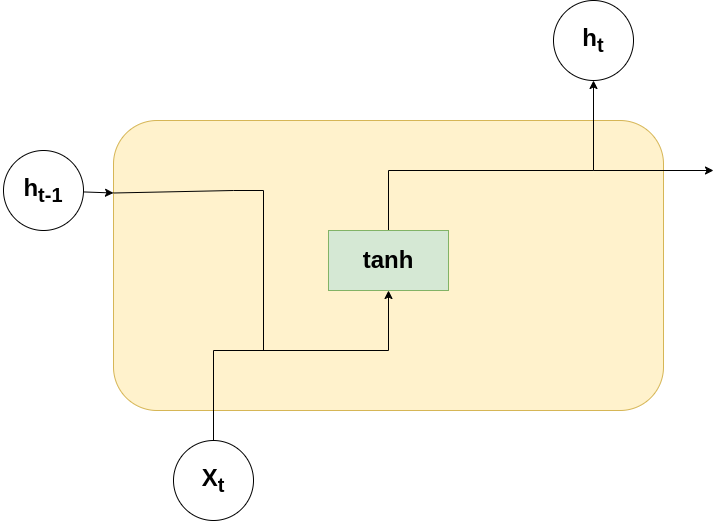
\includegraphics[scale=0.4]{figures/rnn.drawio.png}
    \caption{Example of a RNN Cell. The activation function, $tanh$ in this example, can be switched out for another activation function.}
    \label{fig:rnncell}
\end{figure}


Typically, \acrshort{relu} is used as the activation function in these networks, as it is cheap to perform and we don't need more expressive activation functions. Other common activation functions are sigmoid and tanh. 

$$g(z) = max(0, z)$$
$$g(z) = \frac{1}{1 + e^{-z}}$$
$$g(z) = \frac{e^z - e^{-z}}{e^z + e^{-z}}$$

Although \acrshort{rnn}s have several advantages, they are highly prone to both vanishing gradients as well as exploding gradients. These occur when the gradients become so small they essentially disappear through the iterations of backpropagation. \\ 



Recurrent Batch Normalization
\begin{equation} \label{eq:bnrnn}
    BN(\textbf{h}; \gamma, \beta) = \beta + \gamma \circ \frac{
    \textbf{h} - \hat{E}[\textbf{h}]
    }{
    \sqrt{\hat{Var} [\textbf{h}] + \epsilon}
    }
\end{equation}
